%%%%%%%%%%%%%%%%%%%%%%%%%%%%%%%%%%%%%%%%%%%%%%%%%%%%%%%%%%%%%%%%%%%%%%
% LaTeX Template: Project Titlepage
%
% Source: http://www.howtotex.com
% Date: April 2011
% 
% This is a title page template which be used for articles & reports.
% 
% Feel free to distribute this example, but please keep the referral
% to howtotex.com
% 
%%%%%%%%%%%%%%%%%%%%%%%%%%%%%%%%%%%%%%%%%%%%%%%%%%%%%%%%%%%%%%%%%%%%%%
% How to use writeLaTeX: 
%s
% You edit the source code here on the left, and the preview on the
% right shows you the result within a few seconds.
%
% Bookmark this page and share the URL with your co-authors. They can
% edit at the same time!
%
% You can upload figures, bibliographies, custom classes and
% styles using the files menu.
%
% If you're new to LaTeX, the wikibook is a great place to start:
% http://en.wikibooks.org/wiki/LaTeX
%
%%%%%%%%%%%%%%%%%%%%%%%%%%%%%%%%%%%%%%%%%%%%%%%%%%%%%%%%%%%%%%%%%%%%%%
%
% --------------------------------------------------------------------
% Preamble
% --------------------------------------------------------------------
\documentclass[paper=a4, fontsize=10pt]{scrartcl}	% KOMA
\usepackage[bottom=1.1in, top=0.9in]{geometry}
\usepackage{lmodern}

\newcommand{\specialcell}[2][c]{%
	\begin{tabular}[#1]{@{}c@{}}#2\end{tabular}}
\usepackage{todonotes}
\usepackage{listings}
\usepackage{graphbox}
\usepackage{hyperref}
\usepackage{twoopt}
\usepackage{adjustbox}
\usepackage[english]{babel}
\usepackage{graphicx}
\usepackage{subcaption}
\usepackage{pgfplots}
\usepackage{mwe}
\usepackage{color, colortbl}
\usepackage[protrusion=true,expansion=true]{microtype}	
\usepackage{amsmath,amsfonts,amsthm,amssymb}
\usepackage{tabularx}
\usepackage{float}

\usepackage{lmodern}

\usepackage{todonotes}
\usepackage{listings}
\usepackage{graphbox}
\usepackage{hyperref}
\usepackage{twoopt}
\usepackage{adjustbox}
\usepackage[english]{babel}
\usepackage{graphicx}
\usepackage{subcaption}
\usepackage{mwe}
\usepackage{color, colortbl}
\usepackage[protrusion=true,expansion=true]{microtype}	
\usepackage{amsmath,amsfonts,amsthm,amssymb}
\usepackage{tabularx}
\usepackage{float}
\usepackage{tikz} 
\usepackage{xcolor}
\usepackage{listings}
\usepackage{arydshln}
\usepackage{bytefield}

\definecolor{mGreen}{rgb}{0,0.6,0}
\definecolor{mGray}{rgb}{0.5,0.5,0.5}
\definecolor{mPurple}{rgb}{0.58,0,0.82}
\definecolor{backgroundColour}{rgb}{0.95,0.95,0.92}

\newcommand\setrow[1]{\gdef\rowmac{#1}#1\ignorespaces}
\newcommand\clearrow{\global\let\rowmac\relax}
\usepackage{graphicx}
\usepackage[T1]{fontenc}
\definecolor{Red}{rgb}{1,0.7,0.7}
\definecolor{Yellow}{HTML}{FAFAD2}
\definecolor{Green}{HTML}{9ACD32}
\definecolor{Blue}{rgb}{0.5,0.8,1}
\lstset{
	frame=single,
	xleftmargin=15pt,
	xrightmargin=15pt,
	basicstyle=\ttfamily\small
}
\lstdefinestyle{CStyle}{
	backgroundcolor=\color{backgroundColour},   
	commentstyle=\color{mGreen},
	keywordstyle=\color{magenta},
	numberstyle=\tiny\color{mGray},
	stringstyle=\color{mPurple},
	basicstyle=\footnotesize,
	breakatwhitespace=false,         
	breaklines=false,                 
	captionpos=b,                    
	keepspaces=true,                 
	numbers=left,                    
	numbersep=5pt,                  
	showspaces=false,                
	showstringspaces=false,
	showtabs=false,                  
	tabsize=2,
	language=C
}
\lstset{basicstyle=\ttfamily,
	showstringspaces=false,
	commentstyle=\color{red},
	keywordstyle=\color{blue}
}


\usepackage{graphicx}
\usepackage[T1]{fontenc}
\definecolor{Red}{rgb}{1,0.7,0.7}
\definecolor{Yellow}{HTML}{FAFAD2}
\definecolor{Green}{HTML}{9ACD32}
\definecolor{Blue}{rgb}{0.5,0.8,1}
\lstset{
	backgroundcolor=\color{backgroundColour},   
	commentstyle=\color{mGreen},
	keywordstyle=\color{magenta},
	numberstyle=\tiny\color{mGray},
	stringstyle=\color{mPurple},
	basicstyle=\footnotesize,
	breakatwhitespace=false,         
	breaklines=false,                 
	captionpos=b,                    
	keepspaces=true,                 
	numbers=left,                    
	numbersep=5pt,                  
	showspaces=false,                
	showstringspaces=false,
	showtabs=false,                  
	tabsize=2,
	frame=single,
	xleftmargin=15pt,
	xrightmargin=15pt,
	basicstyle=\ttfamily\small
}
% --------------------------------------------------------------------
% Definitions (do not change this)
% --------------------------------------------------------------------
\newcommand{\HRule}[1]{\rule{\linewidth}{#1}} 	% Horizontal rule
\newcommandtwoopt*{\myref}[3][][]{%
	\hyperref[{#3}]{%
		\ifx\\#1\\%
		\else
		#1~%
		\fi
		\ref*{#3}%
		\ifx\\#2\\%
		\else
		\,#2%
		\fi
	}%
}

\makeatletter							% Title
\def\printtitle{%						
	{\centering \@title\par}}
\makeatother									

\makeatletter							% Author
\def\printauthor{%					
	{\centering \large \@author}}				
\makeatother							

% --------------------------------------------------------------------
% Metadata (Change this)
% --------------------------------------------------------------------
\title{	\normalsize \textsc{Politecnico di Torino\\GPU Programming} 	% Subtitle
	\\[2.0cm]								% 2cm spacing
	\HRule{0.5pt} \\						% Upper rule
	\LARGE \textbf{\uppercase{Assignment:\\CUDA Video Streaming}}	% Title
	\HRule{2pt} \\ [0.5cm]		% Lower rule + 0.5cm spacing
	\normalsize 
	\today % Todays date
}

\author{
	Group 16
}

\begin{document}
	% ------------------------------------------------------------------------------
	% Maketitle
	% ------------------------------------------------------------------------------
	\thispagestyle{empty}		% Remove page numbering on this page
	
	\printtitle					% Print the title data as defined above
	\vfill
	\printauthor				% Print the author data as defined above
	\newpage
	% ------------------------------------------------------------------------------
	% Begin document
	% ------------------------------------------------------------------------------
	\setcounter{page}{1}		% Set page numbering to begin on this page
	\section{Introduction}
	
	
	\section{HeatMap}
	Since the basis of this project is to send the pixel difference, the lower the dissimilarities the higher the bandwidth saving. So, in order to better visualize which pixels changes the most and the different magnitudes, an heatmap is generated with the current and the previous frames.
	
	A heat map is nothing else than a data visualization technique represents the magnitude of a measurement as color in two dimensions, in this case an image. The idea is first compute the difference between two successive frames and then represent it using a color scale from blue to red, where blue means low difference and red high difference. The Image \ref{fig:heat_v0} shows a naif implementation of heat map, available at \texttt{heat\_map\_benchmark/v0.cu}, that generates in real time the image on the right.


	\begin{figure}[H]
		\centering
		\includegraphics[width=0.9\linewidth]{images/heatmap/v0}
		\caption{\textit{Example of real-time heat map from webcam}}
		\label{fig:heat_v0}
	\end{figure}
	The first \textit{naif} version is running on the CPU and can generate an heatmap in more or less 980ms, that is too much. This is also due to the complexity of the function itself that is used to map a normalized pixel difference to a blue-red scale.\newline\newline
	All programs versions for the heat map are available in the \texttt{heat\_map\_benchmark} folder.
	
	\subsection{Heat map pixel mapping - CPU Naif implementation}
	In order to convert the difference of a pixel into the three color component (RGB), the usage of the \textit{sine} function has been done. The difference of the each pixel has been computed as the sum of the absolute value of the difference of the single color component, as:
	\[
		diff = abs(Previous[i,R] - Curr[i,R]) + abs(Previous[i,G] - Curr[i,G] + abs(Previous[i,B] - Curr[i,B])
	\]
	Where the $Previous[i,R]$ is the pixel red color component of the pixel at index $i$. In the worst case, a pixel can be turned from black to withe or vice versa and so, the $0 \leq diff \leq 765$, that is $255 \cdot 3$. Then the $diff$ value is taken and normalize, by using 765 so that, $0 \leq diff_{norm} \leq 1$.:
	\[
		diff_{norm} = \frac{diff}{765}
	\]
	
	This value must be mapped into the tree RGB component of the heat map; the pixel must be more blue if the difference is more toward 0.0, yellow/green if near 0.5 and red if next to 1.0.
	The smoothed way to perform this task is to use three different sine function, centered respectively on 0.0, 0.5 and 1.0 as in the following way:
	\begin{align*}
		\text{RED    } & \quad sin(\pi \cdot diff_{norm} - \frac{\pi}{2.0})\\
		\text{GREEN  } & \quad sin(\pi \cdot diff_{norm})\\
		\text{BLUE   } & \quad sin(\pi \cdot diff_{norm} + \frac{\pi}{2.0})
	\end{align*}
	The plot of the three sine functions is available at Figure \ref{fig:heat_sine}.

	 
	\begin{figure}[H]
		\centering
		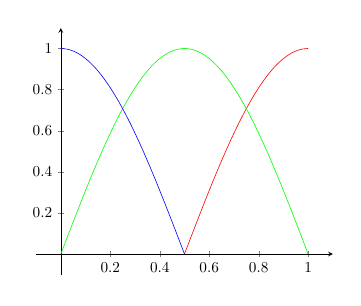
\begin{tikzpicture}[scale=0.55]
			\begin{axis}[
				trig format plots=rad,
				axis lines = middle,
				enlargelimits,
				clip=false
				]
				\addplot[domain=0.5:1,samples=200,red] {sin(pi*x - pi/2.0)};
				\addplot[domain=0:1,samples=200,green] {sin(x*pi)};
				\addplot[domain=0:0.5,samples=200,blue] {sin(pi*x + pi/2.0)};
				
			\end{axis}
		\end{tikzpicture}
	\caption{\textit{Mapping function from pixel difference to RGB components}}
	\label{fig:heat_sine}
	\end{figure}
	The CPU implementation is the following:
	\begin{lstlisting}[style=CStyle]
struct HeatElemt {
	int r;
	int g;
	int b;
};

HeatElemt getHeatPixel(int diff){
	struct HeatElemt h;
	float diff1 = diff/(255.0*2.0);
	
	// Map the difference into the three color components
	h.r = min(max(sin(M_PI*diff1 - M_PI/2.0)*255.0, 0.0),255.0);
	h.g = min(max(sin(M_PI*diff1)*255.0, 0.0),255.0);
	h.b = min(max(sin(M_PI*diff1 + M_PI/2.0)*255.0, 0.0),255.0);
}

while (1) {
	cap >> image2;
	for (int y = 0; y < H; y++){
		for (int x = 0; x < W; x++){
			Vec3b & intensity = image1.at<Vec3b>(y, x);
			Vec3b a = image1.at<Vec3b>(y, x);
			Vec3b b = image2.at<Vec3b>(y, x);
			
			// Compute the absolute difference
			HeatElemt elem = getHeatPixel(abs(a.val[0] - b.val[0]) + 
			abs(a.val[1] - b.val[1]) + abs(a.val[2] - b.val[2]));
			
			intensity.val[0] = elem.b;
			intensity.val[1] = elem.g;
			intensity.val[2] = elem.r;
		}
	}
	image1 = image2.clone();
}\end{lstlisting}
	
	
	\subsection{CUDA heat map implementation}
	
	The idea is to rewrite what described in the previous section into a CUDA code. The GPU allows to run in parallel multiple instance of the same kernel, so that the execution can be done in parallel in order to speed up the computation.
	
	This is exactly what the next section will explain. The kernel call allows to configure how many thread per kernel will be executed; obviously, depending on that number, the accessed locations must be defined accordingly. In fact, by defining $K$ the number of thread lunched, each thread will work on a specific portion of the entire image:
	\[
		\text{Thread portion dimension} = \frac{W \cdot H \cdot 3}{K}
	\]
	Where $W$ and $H$ are the width and height of the image. 
	
	\subsubsection{CUDA first naif version}
	The first implementation of the algorithm in CUDA is based on a 1:1 transposition of what done in the CPU, in the GPU. Always using OpenCV, two next frames are fetched, send to the kernel and the heat map computed.\newline\newline
	Unfortunately, the type of the problem doesn't need any shared or constant memory because each location in the image (all three colors of all pixels) are accessed only one and using a shared memory would have only reduced the performance due to an useless copy and there are not portion of constant memory.
	
	CUDA allows to get the information about the maximum number of thread by using the \texttt{cudaGetDeviceProperties} command. Having the maximum number of thread, it's possible to call the kernel in the following way:
	\begin{lstlisting}[style=CStyle]
// Kernel per block computation
cudaGetDeviceProperties(&prop, 0);
int threads = prop.maxThreadsPerBlock;

// Copy from Host to Device
cudaMemcpy(d_prev, image1,  W*H*C * sizeof *image1, cudaMemcpyHostToDevice);
cudaMemcpy(d_curr, image2,  W*H*C * sizeof *image2, cudaMemcpyHostToDevice);

kernel<<<1, threads>>>(d_curr, d_prev, (W*H*C)/threads, d_out);

// Copy heat map from Device to Host
cudaMemcpy(heatmap, d_out, W*H*C * sizeof *heatmap, cudaMemcpyDeviceToHost);\end{lstlisting}
	
	An extensive analysis of the correct number of threads has been done at Section \ref{sec:thread_n}.\newline\newline
	In order to speed up the data management, instead of copying into a support array of \texttt{uint8\_t} the entire two frames (previous and current), both frames are directly copied into the device buffers with the \texttt{cudaMemcpy} procedure. 
	
	The GPU implementation of the first CUDA code is the following:
	\begin{lstlisting}[style=CStyle]
__global__ void kernel(uint8_t *current, uint8_t *previous,
					int maxSect, uint8_t* d_heat_pixels) {
	
	// Index relative to the block					
	int x = threadIdx.x + blockDim.x * blockIdx.x;
	
	// Start of the sector for this thread
	int start = x * maxSect;
	int max = start + maxSect;
	for (int i = start; i < max; i=i+C) {
		
		// Compute the pixel difference
		int pixelDiff = fabsf(current[i] - previous[i]) + fabsf(current[i+1]
				- previous[i+1]) + fabsf(current[i+2] - previous[i+2]); 
		float diff1 = pixelDiff/(255*2.0);
		
		// Map different into the three color component
		int r = fminf(fmaxf(sinf(M_PI*diff1 - M_PI/2.0)*255.0, 0.0),255.0);
		int g = fminf(fmaxf(sinf(M_PI*diff1)*255.0, 0.0),255.0);
		int b = fminf(fmaxf(sinf(M_PI*diff1 + M_PI/2.0)*255.0, 0.0),255.0);
		d_heat_pixels[i] = b;
		d_heat_pixels[i+1] = g;
		d_heat_pixels[i+2] = r;
	}
} \end{lstlisting}
	
	After having run the \texttt{nvprof}, the main contribution to the execution time from the profiler are:
	\begin{figure}[H]
		\centering
			\begin{center}
			\begin{tabular}{ |c|c|c|c| } 
				\hline
				\textbf{Type} & \textbf{Time} (\%) & \textbf{Avg} & \textbf{Name} \\ 
				\hline
				GPU activities & 86.14 & 49.958 & kernel \\ 
				& 9.38 & 2.5577ms & [CUDA memcpy HtoD] \\ 
				& 4.48 & 2.4427ms & [CUDA memcpy DtoH] \\ 
				\hline
				API calls & 93.88 & 18.820ms & cudaMemcpy \\ 
				& 5.88 & 181.61ms & cudaMalloc \\ 
				\hline
			\end{tabular}
		\end{center}
		\label{fig:table_v1}
		\caption{\textit{Profiling result v1.cu}}
	\end{figure}
	In fact, the cumulative time needed to copy all two frames into the device, execute the kernel and copy back the image in order to display it, takes approximately 57ms. 
	
	\subsubsection{CUDA switching frames}
	
	Instead of copying each time both the two frame, one of the two can be reused by only switching the two points, so that the one that previously was the current will became the previous; at this point, only the new frame must be copied into the device memory. This means that approximately the \textit{CUDA memcpy HtoD} should be half of the previous time. This led to a \texttt{v2.cu} implementation, that exploit this pointer switching to reduce the memory transfer. The below code portion shows only the pointer switching in the loop used to fetch the frames.
		\begin{lstlisting}[style=CStyle]
while(1){
	// New frame fetch
	cap >> image2;
	
	// Pointer switching
	uint8_t* tmp = d_curr;
	d_curr = d_prev;
	d_prev = tmp;
	
	// Kernel call
	cudaMemcpy(d_curr, image2,  W*H*C * sizeof *image2, cudaMemcpyHostToDevice);
	kernel<<<1, threads>>>(d_curr, d_prev, (W*H*C)/threads, d_out);
	cudaMemcpy(heatmap, d_out, W*H*C * sizeof *heatmap, cudaMemcpyDeviceToHost);
	
	image1 = image2.clone();
}\end{lstlisting}
	
	\begin{figure}[H]
		\centering
		\begin{center}
			\begin{tabular}{ |c|c|c|c| } 
				\hline
				\textbf{Type} & \textbf{Time} (\%) & \textbf{Avg} & \textbf{Name} \\ 
				\hline
				GPU activities & 90.54 & 46.023 & kernel \\ 
				& 4.85 & 2.4400ms & [CUDA memcpy HtoD] \\ 
				& 4.61 & 2.3453ms & [CUDA memcpy DtoH] \\ 
				\hline
				API calls & 89.88 & 26.026ms & cudaMemcpy \\ 
				& 9.90 & 192.15ms & cudaMalloc \\ 
				\hline
			\end{tabular}
		\end{center}
		\label{fig:table_v2}
		\caption{\textit{Profiling result v2.cu}}
	\end{figure}
	The average kernel execution time is in ms, and it is not a figure of interest, since it is more or less equal to the previous version. What is important is that now, the percentage of time used for the kernel is increase, due to the reduced \textit{CUDA memcpy HtoD} (from  9.38\% to 4.85\%). This means that the GPU will analyze more frame in the same time frame. As we would expect, now the time needed to copy a frame from the memory to the device, execute the kernel and then retrieve the heat map takes about 50ms (12\% faster).
	
	\subsubsection{CUDA access at the int level instead of uint8\_t}
	In order to reduce the number of accesses to memory, the idea was to access at the int level instead of the byte level. This means that frame information are still copied from host to device as arrays of bytes but they are accesses at the int level. So, if the current and the previous frames are passed as \texttt{uint8\_t *current, uint8\_t *previous}, the access is aligned at the 4 bytes. 
	Another problem arises: the threads now access the memory with a granularity of 4 byte, but since the pixel difference needs needs only the first three bytes (RGB), in order to optimize and avoid to read twice from the memory, colors are read only once every 3 bytes. So, when the position of the color in the image is the first, the colors of the heat map are set in the current and next two bytes of the output array, accordingly to the computed difference.
	\begin{lstlisting}[style=CStyle]
__global__ void kernel(uint8_t *current, uint8_t *previous,
					int maxSect, uint8_t* d_heat_pixels) {
	int x = threadIdx.x + blockDim.x * blockIdx.x;
	int start = x * maxSect;
	int max = start + maxSect;
	int cc, pc;
	for (int i = start; i < max; i++) {
		
		// Access one 4 byte at a time
		cc = ((int *)current)[i];
		pc = ((int *)previous)[i];
		int pixelDiff = 0;
		for (int j = 0; j < 4; j++) {
			
			// Conversion from difference to heat map only every 3 bytes
			if((i*4+j) % 3 == 0){
				int pixelDiff = fabsf(((uint8_t *)&cc)[j] - ((uint8_t *)&pc)[j]) +
				fabsf(((uint8_t *)&cc)[j+1] - ((uint8_t *)&pc)[j+1]) +
				fabsf(((uint8_t *)&cc)[j+2] - ((uint8_t *)&pc)[j+2]);
				float diff1 = pixelDiff/(255*2.0);
				int r = fminf(fmaxf(sinf(M_PI*diff1 - M_PI/2.0)*255.0, 0.0),255.0);
				int g = fminf(fmaxf(sinf(M_PI*diff1)*255.0, 0.0),255.0);
				int b = fminf(fmaxf(sinf(M_PI*diff1 + M_PI/2.0)*255.0, 0.0),255.0);
				d_heat_pixels[i*4+j] = b;
				d_heat_pixels[i*4+j+1] = g;
				d_heat_pixels[i*4+j+2] = r;
				
				// Reset the pixel difference
				pixelDiff = 0;
			}
		}
	}
}\end{lstlisting}
	Since now each threads works on 4 bytes, the dimension of the data that each block must work on is reduced by $1/4$, as in the following way:
		\begin{lstlisting}[style=CStyle]
cudaGetDeviceProperties(&prop, 0);
int threads = prop.maxThreadsPerBlock;

cudaMemcpy(d_curr, image2,  W*H*C * sizeof *image2, cudaMemcpyHostToDevice);

// Kernel call /4
kernel<<<1, threads>>>(d_curr, d_prev, ((W*H*C)/threads)/4, d_out);
cudaMemcpy(heatmap, d_out, W*H*C * sizeof *heatmap, cudaMemcpyDeviceToHost);\end{lstlisting}

	This led to another version, available at \texttt{v3.cu} allows to obtain the following results:
	\begin{figure}[H]
		\centering
		\begin{center}
			\begin{tabular}{ |c|c|c|c| } 
				\hline
				\textbf{Type} & \textbf{Time} (\%) & \textbf{Avg} & \textbf{Name} \\ 
				\hline
				GPU activities & 84.08 & 25.457ms & kernel \\ 
				& 8.14 & 2.4405ms & [CUDA memcpy HtoD] \\ 
				& 7.78 & 2.3549ms & [CUDA memcpy DtoH] \\ 
				\hline
				API calls & 85.73 & 15.810ms & cudaMemcpy \\ 
				& 13.93 & 172.12ms & cudaMalloc \\ 
				\hline
			\end{tabular}
		\end{center}
		\label{fig:table_v3}
		\caption{\textit{Profiling result v3.cu}}
	\end{figure}
	
	This version allows to copy the next frame from memory to device, execute the kernel and retrieve the result in about 30ms (about 40\% of performance increase from \texttt{v2.cu}). This is highlighted in the table by the average time needed to execute the kernel itself, we went from 46.023ms to 25.457ms, thanks to the reduce access time to the memory.
	
	\subsection{Evaluation of the number of threads}
	\label{sec:thread_n}
	For a first implementation, the number of thread has been set to the maximum allowable from the architecture, that is given by the \texttt{cudaGetDeviceProperties} CUDA function in order to make the program independent form the device used. For example, for the Jetson Nano, the maximum number of threads are 1024.\newline\newline
	In order to understand how the number of threads impacts on the heat map generation, a bash script has been build in order to dynamically change the $K$ parameter via compiler directive. The number of threads must be a multiple of 4, so that the array of the pixels can be divided into portion in such a way that a pixel is not split between two kernel.
	
	This is the bash code to execute the 
	\begin{lstlisting}[language=bash]
#!/bin/bash
for i in {1..256}
do
	k=$(( 4*i ))
	
	# Profiler call
	avg=`sudo /usr/local/cuda/bin/nvprof ./heatMap $k 2>&1`
	
	# Data extraction
	kern=`echo "$avg" | grep kernel | awk '{print $6}'`
	kernt=`echo "$avg" | grep kernel | awk '{print $4}'`
	hd1=`echo "$avg" | grep "CUDA memcpy HtoD" | awk '{print $4}'`
	hd2=`echo "$avg" | grep "CUDA memcpy HtoD" | awk '{print $2}'`
	dh1=`echo "$avg" | grep "CUDA memcpy DtoH" | awk '{print $4}'`
	dh2=`echo "$avg" | grep "CUDA memcpy DtoH" | awk '{print $2}'`
	echo "$k $all $kern $kernt $hd1 $hd2 $dh1 $dh2" >> times.txt
done\end{lstlisting}
	In this way, the output of the profiler and the time needed to copy the frame, generate the heat map and retrieve the result is parsed and wrote into a file called \texttt{times.txt}. Thanks to another script, the most useful data are plot.
	
	\begin{figure}[H]
		\centering
		\begin{subfigure}{.45\textwidth}
			\centering
			\includegraphics[width=.8\linewidth]{images/heatmap/plot_kernel_times.png}
			\caption{Time needed to perform an heatmap depending on the number of kernel set}
			\label{fig:sub1}
		\end{subfigure}%
		\hspace{5mm}
		\begin{subfigure}{.45\textwidth}
			\centering
			\includegraphics[width=.8\linewidth]{images/heatmap/hd.png}
			\caption{Time needed to copy from Host to Device (blue) and from Device to Host (orange)}
			\label{fig:sub2}
		\end{subfigure}
	\end{figure}
	This is not the behaviour that we would have expected, beside the time needed to copy is more or less constant, by increasing the number of threads for that kernel we would expect that the time needed for the heat map computation would be lower. This is probably due to the fact that the \textit{warp} has a fixed size of 32 threads and, even if by increasing the number of thread its execution time is lower, their management probably introduce too much overhead to obtain benefits.
	
	Beside this, the time needed to perform an heatmap vs the number of threads, shows a peculiar behaviour. After about $N > 280$ the times tend to oscillate between more or less 50ms and 27ms. Even if this seems not a big difference, in the filed of real-time image processing, it's a huge improvement. In order to avoid errors, the same script has been run multiple times and the results is always the same. Since the internal infrastructure is a black box, the hardware probably manage in different ways the threads with the respect to their number.\newline
	The best observed thread configuration for the Jetson Nano, seems to be 716.\newline\newline
	In fact, by running the same exact algorithm describe before but the number of threads is set to 718 (that is the best kernel accordingly to the plot above), the time needed to copy a frame, compute the heat map and then copy back the heat map matrix is about 27ms. This leads to a increasing of performance of 10\%, that in this domain is not negligible.
	
	The following table shows some meaningful data extracted from the profiler:
		\begin{figure}[H]
		\centering
		\begin{center}
			\begin{tabular}{ |c|c|c|c| } 
				\hline
				\textbf{Type} & \textbf{Time} (\%) & \textbf{Avg} & \textbf{Name} \\ 
				\hline
				GPU activities & 84.30 & 24.380ms & kernel \\ 
				& 8.04 & 2.4599ms & [CUDA memcpy HtoD] \\ 
				& 7.66 & 2.383ms & [CUDA memcpy DtoH] \\ 
				\hline
				API calls & 90.06 & 16.192ms & cudaMemcpy \\ 
				& 9.57 & 115.27ms & cudaMalloc \\ 
				\hline
			\end{tabular}
		\end{center}
		\label{fig:table_v4}
		\caption{\textit{Profiling result v3.cu}}
	\end{figure}

	By considering only the CUDA algorithm, the optimizations show decreasing fashion of the needed to process the two frames and generate the heat map. The Loop average time, is the time needed to copy the image from the Host to the Device, summed to the heat map time computation and the time needed to copy it back. On the other hand, the plot on the right shows only the average kernel time. All data are in ms. 
	\begin{center}
		\includegraphics[width=0.65\linewidth]{images/heatmap/histo_results}
	\end{center}
	
	
	\section{Noise filtering}
	
	
	A second implementation, that is used to speed up the computation is to turn in red all pixels that are above a certain threshold. Obviously, the complexity of this computation is much easier than the previous one and in the CPU allows to compute that kind of map in around 300ms.
	\begin{figure}[H]
		\centering
		\includegraphics[width=0.4\linewidth]{images/heatmap/v0-red}
		\caption{\textit{All non normalized pixel difference are turned to red if above a certain threshold, in this case 30}}
		\label{fig:v0-red}
	\end{figure}
	
	The two implementations are manged via some compiler directives that allows to increase the performance, since only one of them can be visualized. The purpose of them is completely different, since the original heat map, the one explained at the beginning is used to understand the magnitude of the pixel difference while the second one (the black-red) is used to better visualize the noise pixels, by using a threshold. This allows to have a visual evaluation of the noise filter, that will be explained in the next section.
	
\end{document}